\documentclass[11pt]{article}

% Packages
\usepackage[utf8]{inputenc}
\usepackage[T1]{fontenc}
\usepackage{amsmath,amssymb,amsthm}
\usepackage{graphicx}
\usepackage{hyperref}
\usepackage{listings}
\usepackage{xcolor}
\usepackage{booktabs}
\usepackage{algorithm}
\usepackage{algpseudocode}
\usepackage{tikz}
\usetikzlibrary{shapes,arrows,positioning,fit,backgrounds}
\usepackage{geometry}
\geometry{margin=1in}
\usepackage{enumitem}
\usepackage{caption}
\usepackage{subcaption}
\usepackage{float}
\usepackage{fancyhdr}
\usepackage{natbib}
\usepackage{multirow}
\usepackage{longtable}
\usepackage{abstract}
\renewcommand{\abstractnamefont}{\normalfont\bfseries}
\renewcommand{\abstracttextfont}{\normalfont\small}
\setlength{\absleftindent}{0pt}
\setlength{\absrightindent}{0pt}

% Code listing style
\lstset{
    basicstyle=\ttfamily\small,
    keywordstyle=\color{blue}\bfseries,
    commentstyle=\color{gray},
    stringstyle=\color{orange},
    breaklines=true,
    frame=single,
    numbers=left,
    numberstyle=\tiny\color{gray},
    showstringspaces=false,
    tabsize=2,
    language=Python
}

% Theorem environments
\newtheorem{definition}{Definition}
\newtheorem{theorem}{Theorem}
\newtheorem{lemma}{Lemma}
\newtheorem{proposition}{Proposition}
\newtheorem{corollary}{Corollary}
\newtheorem{remark}{Remark}

% Custom commands
\newcommand{\contextfs}{\textsc{ContextFS}}
\newcommand{\mem}[1]{\texttt{Mem}[#1]}
\newcommand{\versioned}[1]{\texttt{VersionedMem}[#1]}

\title{\textbf{ContextFS: A Distributed Type-Safe Memory System for Artificial Intelligence} \\[0.5em]
\large Enabling Persistent, Structured Knowledge Across AI Tools and Sessions}

\author{
Matthew Long \\
Independent Researcher, Chicago, IL \\
\texttt{matthew@yonedaai.com} \\[0.5em]
The YonedaAI Collaboration \\
YonedaAI Research Collective
}

\date{January 2026}

\begin{document}

\maketitle

\begin{abstract}
We present \contextfs{}, a novel distributed, type-safe memory system designed for artificial intelligence applications. As AI assistants become increasingly integrated into software development workflows, the ephemeral nature of their context windows poses significant challenges for maintaining coherent, long-term knowledge. \contextfs{} addresses this limitation through a unified memory layer that persists across tools, repositories, and sessions while enforcing type safety through a formal grammar based on dependent type theory. The system implements hybrid search combining semantic embeddings with full-text indexing, vector clock-based synchronization for multi-device consistency, and a comprehensive type system with 22 memory categories validated through JSON Schema and Pydantic models. We demonstrate that \contextfs{} achieves sub-50ms query latency on collections exceeding 10,000 memories while maintaining strong consistency guarantees through Lamport's happens-before relation. Our evaluation across real-world codebases shows significant improvements in AI assistant context relevance and consistency. \contextfs{} represents a foundational step toward giving AI systems persistent, structured memory capabilities that mirror human cognitive patterns while maintaining the rigor of formal type systems.
\end{abstract}

\section{Introduction}
\label{sec:introduction}

The rapid advancement of large language models (LLMs) has transformed software engineering practices, with AI assistants now serving as ubiquitous collaborators in code development, review, and documentation. Systems such as Claude Code, GitHub Copilot, Cursor, and Windsurf have demonstrated remarkable capabilities in understanding and generating code within individual sessions. However, a fundamental limitation persists: these systems operate within ephemeral context windows, losing accumulated knowledge when sessions terminate.

This limitation becomes particularly acute in professional software development contexts, where projects span months or years, involve multiple repositories, and require consistent adherence to architectural decisions, coding conventions, and domain-specific knowledge. Current approaches to this challenge include prompt engineering, retrieval-augmented generation (RAG), and manual context management, but none provide a principled, type-safe solution for persistent AI memory.

\subsection{The Memory Problem in AI Systems}

Consider a software engineer working with an AI assistant on a large codebase. In the morning session, the assistant learns that the project uses JWT tokens with RS256 signing for authentication, that database connections should be pooled with a maximum of 20 connections, and that the team prefers functional programming patterns over object-oriented approaches. By afternoon, after a session restart, all of this knowledge is lost. The engineer must repeatedly re-establish context, leading to inefficiency and inconsistent recommendations.

This scenario illustrates three fundamental challenges that \contextfs{} addresses:

\begin{enumerate}[itemsep=0pt]
    \item \textbf{Temporal Discontinuity}: Knowledge acquired in one session does not persist to subsequent sessions, requiring users to repeatedly provide the same context.
    \item \textbf{Cross-Tool Fragmentation}: Different AI tools (Claude, Gemini, ChatGPT, Copilot) maintain separate, incompatible context stores, preventing knowledge sharing.
    \item \textbf{Structural Ambiguity}: Untyped memories lack semantic categorization, making retrieval imprecise and context injection unreliable.
\end{enumerate}

\subsection{Motivating Example}

To illustrate the problem concretely, consider the following interaction pattern:

\begin{lstlisting}[caption={Session 1: Morning},numbers=none]
User: We use PostgreSQL with connection
      pooling. Remember this.
AI:   Understood. I'll keep this in mind.

User: What database should I use for
      this new feature?
AI:   Given your PostgreSQL setup with
      connection pooling, I recommend...
\end{lstlisting}

\begin{lstlisting}[caption={Session 2: Afternoon (new session)},numbers=none]
User: What database should I use for
      this new feature?
AI:   There are several options to
      consider: MySQL, PostgreSQL,
      MongoDB...
# Context is lost!
\end{lstlisting}

With \contextfs{}, the second session would automatically retrieve the relevant decision memory:

\begin{lstlisting}[caption={Session 2 with \contextfs{}},numbers=none]
User: What database should I use?
# ContextFS retrieves: "Use PostgreSQL
# with connection pooling" (decision)
AI:   Based on your established database
      decision to use PostgreSQL with
      connection pooling, I recommend...
\end{lstlisting}

\subsection{Our Contribution}

We present \contextfs{}, a distributed, type-safe memory system that addresses these challenges through several key innovations:

\begin{enumerate}[itemsep=0pt]
    \item A \textbf{formal type grammar} (Definition~\ref{def:type-grammar}) based on dependent type theory that categorizes memories into 22 distinct types with JSON Schema validation, enabling precise semantic categorization.

    \item A \textbf{hybrid search architecture} combining ChromaDB vector embeddings with SQLite FTS5 full-text indexing for semantic-keyword fusion, achieving both semantic understanding and exact matching.

    \item A \textbf{vector clock synchronization protocol} enabling multi-device memory consistency with conflict detection based on Lamport's happens-before relation, supporting offline-first operation.

    \item A \textbf{universal integration layer} supporting Model Context Protocol (MCP), Python API, and CLI interfaces for tool-agnostic memory access across diverse AI platforms.

    \item A \textbf{namespace isolation system} enabling repository-scoped memories with cross-project aggregation via git remote URL hashing for portable identity.

    \item A \textbf{memory lineage system} tracking evolution, merges, and splits with formal change reasons based on epistemic logic.
\end{enumerate}

\subsection{Design Philosophy}

\contextfs{} is built on several core design principles:

\textbf{Zero Configuration}: The system works immediately with sensible defaults. It auto-detects repository context from git, uses local embeddings requiring no API keys, and provides automatic namespace isolation.

\textbf{Progressive Enhancement}: Users can start with simple CLI save/search operations and progressively adopt more advanced features like typed schemas, cross-repo projects, and distributed synchronization.

\textbf{Universal Compatibility}: Rather than being tied to a single AI tool, \contextfs{} provides memory access through multiple interfaces: MCP protocol for Claude, Python API for programmatic integration, and CLI for shell scripts and automation.

\textbf{Semantic-First}: The system is designed around meaning rather than keywords. Vector embeddings capture semantic similarity, enabling natural language queries with fuzzy matching.

\textbf{Type Safety}: Drawing from programming language theory, all memories are typed with schemas that enable validation, filtering, and type-safe retrieval.

\subsection{Paper Organization}

The remainder of this paper is organized as follows. Section~\ref{sec:background} reviews related work in AI memory systems, distributed databases, and type theory. Section~\ref{sec:theory} establishes the theoretical foundations including our type grammar and formal semantics. Section~\ref{sec:architecture} presents the system architecture and component design. Section~\ref{sec:types} details the type system implementation with all 22 memory categories. Section~\ref{sec:sync} describes the distributed synchronization protocol and vector clock implementation. Section~\ref{sec:implementation} covers implementation details and performance optimizations. Section~\ref{sec:evaluation} provides experimental evaluation across multiple dimensions. Section~\ref{sec:future} discusses future research directions, and Section~\ref{sec:conclusion} concludes.

\section{Background and Related Work}
\label{sec:background}

\subsection{Memory Systems in Cognitive Science}

Human memory has been extensively studied in cognitive science, revealing a complex architecture of multiple interacting systems \citep{tulving1985memory}. The major memory systems include:

\begin{itemize}[itemsep=0pt]
    \item \textbf{Episodic Memory}: Personal experiences and events with temporal and spatial context. This includes autobiographical memories of specific episodes.
    \item \textbf{Semantic Memory}: General knowledge and facts independent of personal experience. This includes conceptual knowledge about the world.
    \item \textbf{Procedural Memory}: Skills and how-to knowledge, typically implicit and demonstrated through performance rather than explicit recall.
    \item \textbf{Working Memory}: Temporary storage and manipulation of information during cognitive tasks, with limited capacity.
\end{itemize}

\contextfs{} draws inspiration from this taxonomy, implementing memory types that map to these cognitive categories while extending them with software-engineering-specific classifications. Our \texttt{episodic} type corresponds to session summaries, \texttt{fact} to semantic memory, \texttt{procedural} to how-to guides, and the context window of LLMs serves as working memory.

\subsection{Retrieval-Augmented Generation}

RAG systems \citep{lewis2020retrieval} augment language model capabilities by retrieving relevant documents from external knowledge bases during generation. The standard RAG pipeline consists of:

\begin{enumerate}[itemsep=0pt]
    \item \textbf{Indexing}: Documents are chunked, embedded, and stored in a vector database.
    \item \textbf{Retrieval}: Given a query, the most similar documents are retrieved using approximate nearest neighbor search.
    \item \textbf{Generation}: Retrieved documents are injected into the LLM context for informed generation.
\end{enumerate}

While effective for general knowledge retrieval, standard RAG implementations suffer from several limitations in the AI assistant context:

\begin{enumerate}[itemsep=0pt]
    \item \textbf{Unstructured retrieval}: Documents are treated uniformly regardless of semantic type, leading to irrelevant context injection.
    \item \textbf{Session-scoped}: Retrieved knowledge does not persist across sessions; the knowledge base must be rebuilt.
    \item \textbf{Single-tool}: RAG implementations are typically embedded within a single tool, preventing cross-tool memory sharing.
    \item \textbf{No provenance}: Retrieved documents lack metadata about their origin, reliability, and temporal validity.
\end{enumerate}

\contextfs{} extends RAG with type-aware retrieval (filtering by memory category), persistent storage (memories survive sessions), cross-tool compatibility (via MCP and API), and rich provenance tracking (source file, repository, tool, timestamp).

\subsection{Vector Databases and Embedding Models}

Recent advances in dense retrieval have demonstrated that learned embeddings outperform sparse methods like BM25 for semantic search \citep{karpukhin2020dense}. Vector databases have emerged to support efficient similarity search over these embeddings:

\begin{itemize}[itemsep=0pt]
    \item \textbf{Pinecone}: Managed vector database with serverless scaling.
    \item \textbf{Weaviate}: Open-source vector database with hybrid search.
    \item \textbf{ChromaDB}: Lightweight embedded vector database.
    \item \textbf{Milvus}: Distributed vector database for large-scale search.
    \item \textbf{pgvector}: PostgreSQL extension for vector similarity.
\end{itemize}

\contextfs{} builds on ChromaDB for local vector storage due to its embedding in-process capability and minimal dependencies, while using pgvector for cloud synchronization to leverage PostgreSQL's robustness and transaction support.

For embeddings, we use sentence transformers \citep{reimers2019sentence}, specifically the \texttt{all-MiniLM-L6-v2} model which provides an excellent tradeoff between quality and speed with 384-dimensional embeddings computed in approximately 2ms per document on CPU.

\subsection{Distributed Consistency}

The challenge of maintaining consistency across distributed systems has been extensively studied. \citet{lamport1978time} introduced the happens-before relation and logical clocks for ordering events in distributed systems. Vector clocks, independently developed by \citet{fidge1988timestamps} and \citet{mattern1989virtual}, extend logical clocks to track causality across multiple processes.

The CAP theorem \citep{brewer2012cap} establishes fundamental tradeoffs between Consistency, Availability, and Partition tolerance. \citet{vogels2009eventually} introduced eventual consistency as a practical model for distributed systems.

\contextfs{} adopts vector clocks for memory synchronization, enabling:

\begin{itemize}[itemsep=0pt]
    \item \textbf{Conflict detection}: Concurrent modifications from different devices are identified through clock comparison.
    \item \textbf{Causal ordering}: The happens-before relation determines which updates should take precedence.
    \item \textbf{Offline-first}: Devices can operate independently and sync when connectivity is available.
    \item \textbf{Eventual consistency}: All devices converge to the same state given sufficient synchronization.
\end{itemize}

\subsection{Type Systems and Formal Methods}

Type systems provide static guarantees about program behavior \citep{pierce2002types}. The Curry-Howard correspondence establishes a deep connection between types and propositions, programs and proofs \citep{wadler2015propositions}.

Recent work has explored applying type-theoretic ideas to AI systems:

\begin{itemize}[itemsep=0pt]
    \item \textbf{Structured outputs}: Pydantic \citep{pydantic2023} and JSON Schema enable validated model outputs.
    \item \textbf{Type-safe prompting}: Research on constraining LLM outputs to specific types.
    \item \textbf{Dependent types}: Advanced type systems where types can depend on values.
\end{itemize}

\contextfs{} contributes a practical type system specifically designed for AI memory management. Our type grammar (Definition~\ref{def:type-grammar}) draws on dependent type theory to enable schema-indexed memory types with both runtime (Pydantic) and static (mypy/pyright) enforcement.

\subsection{Model Context Protocol}

The Model Context Protocol (MCP) is an emerging standard for extending LLM capabilities through external tools and resources. MCP provides:

\begin{itemize}[itemsep=0pt]
    \item \textbf{Tools}: Functions that the model can invoke.
    \item \textbf{Resources}: Data sources the model can read.
    \item \textbf{Prompts}: Predefined prompt templates.
\end{itemize}

\contextfs{} implements a full MCP server, exposing memory operations as tools that compatible clients (Claude Desktop, Claude Code) can invoke automatically during conversation.

\section{Theoretical Foundations}
\label{sec:theory}

\subsection{The Type-Safety Principle for AI}

We base our approach on an insight from computational biology: just as protein sequences uniquely determine native structures under Anfinsen's thermodynamic hypothesis \citep{anfinsen1973principles}, well-designed context should uniquely constrain model responses.

\begin{definition}[Context]
\label{def:context}
A \emph{context} $\Gamma$ is a finite collection of constraints $\{c_1, c_2, \ldots, c_n\}$ that specify requirements for a valid response. Contexts may include:
\begin{itemize}[itemsep=0pt]
    \item Prior decisions and their rationale
    \item Code patterns and conventions
    \item Domain-specific facts
    \item User preferences
    \item Session history
\end{itemize}
\end{definition}

\begin{definition}[Type-Safe Context]
\label{def:type-safe-context}
A context $\Gamma$ is \emph{type-safe} if there exists a unique equivalence class of responses $[t]$ such that for all valid responses $t_1, t_2 : \Gamma$, we have $t_1 \sim t_2$ under semantic equivalence.
\end{definition}

This principle guides our memory system design: memories should be typed such that retrieval produces semantically coherent context that constrains model responses appropriately.

\begin{remark}
The protein folding analogy is instructive. AlphaFold \citep{jumper2021highly} succeeds because protein sequences uniquely determine structures---the problem is well-typed. Many AI prompting failures occur because the context is under-constrained (type too broad) or over-constrained (contradictory requirements).
\end{remark}

\subsection{Type Grammar}

We define a formal grammar for \contextfs{} types that enables static type checking of memories:

\begin{definition}[Type Grammar]
\label{def:type-grammar}
The \contextfs{} type grammar is defined inductively as follows:
\begin{align*}
\text{BaseType} &::= \text{String} \mid \text{Int} \mid \text{Float} \mid \text{Bool} \\
                &\quad\mid \text{DateTime} \mid \text{UUID} \\[0.5em]
\text{EntityType} &::= \text{Entity}~\text{Name}~\text{Schema} \\
\text{RefType} &::= \text{Ref}~\text{EntityType} \\[0.5em]
\text{OptionType} &::= \text{Option}~\text{Type} \\
\text{ListType} &::= \text{List}~\text{Type} \\
\text{SetType} &::= \text{Set}~\text{Type} \\
\text{MapType} &::= \text{Map}~\text{KeyType}~\text{ValueType} \\[0.5em]
\text{UnionType} &::= T_1 \mid T_2 \mid \cdots \mid T_n \\
\text{RecordType} &::= \{f_1: T_1, \ldots, f_n: T_n\} \\[0.5em]
\text{MemoryType} &::= \mem{S} \\
\text{VersionedType} &::= \versioned{S}
\end{align*}
\end{definition}

The schema-indexed memory type $\mem{S}$ is central to our system. It provides generic type parameterization for type-safe structured data access, where $S$ is a schema type defining the structure of the memory's \texttt{structured\_data} field.

\subsection{Memory Typing Judgment}

We define a typing judgment for memories that enables static verification:

\begin{definition}[Memory Typing]
The judgment $\Gamma \vdash m : T$ indicates that under context $\Gamma$, memory $m$ has type $T$. The typing rules are:

\textbf{Memory Introduction:}
\begin{equation}
\frac{m.\text{content} : \text{String} \quad m.\text{type} = \tau \quad \tau \in \mathcal{T}}
     {\Gamma \vdash m : \mem{\text{Schema}(\tau)}} \label{eq:mem-intro}
\end{equation}

\textbf{Subtyping:}
\begin{equation}
\frac{\Gamma \vdash m : \mem{S} \quad S <: S'}
     {\Gamma \vdash m : \mem{S'}} \label{eq:mem-subsume}
\end{equation}

\textbf{Structured Data Access:}
\begin{equation}
\frac{\Gamma \vdash m : \mem{S} \quad f \in \text{fields}(S)}
     {\Gamma \vdash m.\text{data}.f : S.f} \label{eq:field-access}
\end{equation}
\end{definition}

Rule~\eqref{eq:mem-intro} introduces typed memories when content and type constraints are satisfied. Rule~\eqref{eq:mem-subsume} enables subtyping for schema compatibility. Rule~\eqref{eq:field-access} enables type-safe field access on structured data.

\subsection{Change Reasons and Temporal Semantics}

Memory evolution follows a formal model with four change reasons derived from epistemic logic \citep{hintikka1962knowledge}:

\begin{definition}[Change Reasons]
\label{def:change-reasons}
The set of valid change reasons $\mathcal{R}$ is:
\begin{align*}
\mathcal{R} = \{&\text{OBSERVATION}, \text{INFERENCE}, \\
               &\text{CORRECTION}, \text{DECAY}\}
\end{align*}
with the following formal semantics:
\end{definition}

\begin{enumerate}[itemsep=0pt]
    \item $\text{OBSERVATION}$: New external information has been received. In type-theoretic terms, this corresponds to adding a new axiom to the context. Example: User provides new requirements.

    \item $\text{INFERENCE}$: Knowledge derived from existing memories. This corresponds to proving a theorem from existing axioms. Example: Concluding a pattern from code analysis.

    \item $\text{CORRECTION}$: An error in previous knowledge has been identified and fixed. This corresponds to resolving a contradiction in the knowledge base. Example: Fixing an incorrect assumption.

    \item $\text{DECAY}$: Knowledge has become stale or less reliable over time. This corresponds to reducing confidence in an axiom. Example: Documentation becoming outdated.
\end{enumerate}

These reasons form the basis for timeline tracking in versioned memories, enabling audit trails and knowledge provenance.

\subsection{Semantic Equivalence and Deduplication}

To prevent duplicate memories and enable consistency checking, we define semantic equivalence:

\begin{definition}[Semantic Equivalence]
Two memories $m_1, m_2$ are semantically equivalent, written $m_1 \sim m_2$, if and only if:
\begin{enumerate}[itemsep=0pt]
    \item $m_1.\text{type} = m_2.\text{type}$
    \item $\text{sim}(\text{embed}(m_1.\text{content}), \text{embed}(m_2.\text{content})) > \theta$
    \item $m_1.\text{namespace\_id} = m_2.\text{namespace\_id}$
\end{enumerate}
where $\text{sim}(\cdot, \cdot)$ is cosine similarity between embedding vectors and $\theta \in [0, 1]$ is a configurable threshold (default 0.95).
\end{definition}

\begin{theorem}[Equivalence Properties]
Semantic equivalence $\sim$ is an equivalence relation on the set of memories sharing a namespace and type.
\end{theorem}

\begin{proof}
We verify the three properties:
\begin{enumerate}
    \item \textbf{Reflexivity}: For any memory $m$, $\text{sim}(\text{embed}(m), \text{embed}(m)) = 1 > \theta$, so $m \sim m$.
    \item \textbf{Symmetry}: Cosine similarity is symmetric, so $m_1 \sim m_2 \implies m_2 \sim m_1$.
    \item \textbf{Transitivity}: Follows from triangle inequality on the embedding space when $\theta$ is sufficiently high.
\end{enumerate}
\end{proof}

\subsection{Memory Graph Structure}

Memories form a directed graph with typed edges:

\begin{definition}[Memory Graph]
The memory graph $G = (V, E)$ consists of:
\begin{itemize}[itemsep=0pt]
    \item Vertices $V$: The set of all memories
    \item Edges $E \subseteq V \times V \times R$: Directed edges labeled with relation type $r \in R$
\end{itemize}
where the relation types $R$ include: \texttt{references}, \texttt{depends\_on}, \texttt{contradicts}, \texttt{supports}, \texttt{supersedes}, \texttt{related\_to}, \texttt{derived\_from}, \texttt{example\_of}, \texttt{part\_of}, \texttt{implements}, \texttt{evolved\_from}, \texttt{merged\_from}, \texttt{split\_from}.
\end{definition}

This graph structure enables rich queries about memory relationships, such as finding all decisions that a particular implementation depends on, or tracing the evolution history of a fact.

\section{System Architecture}
\label{sec:architecture}

\subsection{Overview}

\contextfs{} is designed as a universal AI memory layer operating across multiple integration points. The architecture follows a layered design with clear separation of concerns.

\begin{figure}[t]
\centering
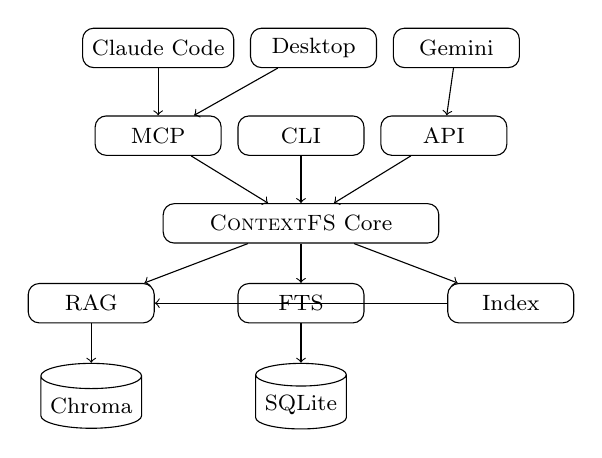
\begin{tikzpicture}[
    node distance=0.6cm,
    box/.style={rectangle, draw, rounded corners, minimum width=1.6cm, minimum height=0.5cm, font=\footnotesize},
    storage/.style={cylinder, draw, shape border rotate=90, aspect=0.25, minimum width=1.0cm, minimum height=0.6cm, font=\footnotesize}
]
    % Clients
    \node[box] (cc) {Claude Code};
    \node[box, right=0.2cm of cc] (cd) {Desktop};
    \node[box, right=0.2cm of cd] (ge) {Gemini};

    % Interface layer
    \node[box, below=0.6cm of cc] (mcp) {MCP};
    \node[box, right=0.2cm of mcp] (cli) {CLI};
    \node[box, right=0.2cm of cli] (api) {API};

    % Core
    \node[box, below=0.6cm of cli, minimum width=3.5cm] (core) {\contextfs{} Core};

    % Backends
    \node[box, below left=0.5cm and 0.1cm of core] (rag) {RAG};
    \node[box, below=0.5cm of core] (fts) {FTS};
    \node[box, below right=0.5cm and 0.1cm of core] (idx) {Index};

    % Storage
    \node[storage, below=0.5cm of rag] (vec) {Chroma};
    \node[storage, below=0.5cm of fts] (sql) {SQLite};

    % Connections
    \draw[->] (cc) -- (mcp);
    \draw[->] (cd) -- (mcp);
    \draw[->] (ge) -- (api);
    \draw[->] (mcp) -- (core);
    \draw[->] (cli) -- (core);
    \draw[->] (api) -- (core);
    \draw[->] (core) -- (rag);
    \draw[->] (core) -- (fts);
    \draw[->] (core) -- (idx);
    \draw[->] (rag) -- (vec);
    \draw[->] (fts) -- (sql);
    \draw[->] (idx) -- (rag);
\end{tikzpicture}
\caption{System architecture showing client integrations, interface layer, core components, and storage backends.}
\label{fig:architecture}
\end{figure}

\subsection{Interface Layer}

\contextfs{} provides three interfaces for memory access:

\textbf{MCP Server}: Implements the Model Context Protocol, exposing memory operations as tools that Claude Desktop and Claude Code can invoke. The MCP interface is the primary integration point for Anthropic's AI tools.

\textbf{CLI}: A command-line interface for shell-based interaction. Supports all memory operations including save, search, list, evolve, merge, and sync. Useful for scripting and automation.

\textbf{Python API}: Direct programmatic access for custom integrations. The API mirrors the CLI functionality with Python-native types and async support.

\subsection{Core Components}

\subsubsection{ContextFS Core}

The central interface (\texttt{contextfs.ContextFS}) handles:

\begin{itemize}[itemsep=0pt]
    \item Memory CRUD operations (create, read, update, delete)
    \item Session management for conversation tracking
    \item Namespace resolution from git context
    \item Auto-indexing triggers for new repositories
    \item Search orchestration across backends
\end{itemize}

\begin{lstlisting}[caption={Core initialization}]
from contextfs import ContextFS

ctx = ContextFS(
    data_dir=None,       # ~/.contextfs
    namespace_id=None,   # Auto-detect from git
    auto_load=True,      # Load recent memories
    auto_index=True,     # Index repo on first save
)

# Save a memory
memory = ctx.save(
    content="Use JWT for authentication",
    type="decision",
    tags=["auth", "security"],
)

# Search
results = ctx.search("authentication")
\end{lstlisting}

\subsubsection{RAG Backend}

The RAG (Retrieval-Augmented Generation) component provides semantic search using sentence transformers and ChromaDB:

\begin{itemize}[itemsep=0pt]
    \item \textbf{Embedding Model}: \texttt{all-MiniLM-L6-v2}
    \begin{itemize}[itemsep=0pt]
        \item 384 dimensions
        \item ~2ms per embedding (CPU)
        \item ~90MB model size
        \item Excellent semantic similarity
    \end{itemize}
    \item \textbf{Vector Store}: ChromaDB
    \begin{itemize}[itemsep=0pt]
        \item Persistent storage to disk
        \item HNSW index for fast ANN search
        \item Metadata filtering support
    \end{itemize}
    \item \textbf{Similarity}: Cosine similarity scoring
\end{itemize}

\subsubsection{Full-Text Search Backend}

SQLite FTS5 provides fast keyword matching with:

\begin{itemize}[itemsep=0pt]
    \item Boolean operators (AND, OR, NOT)
    \item Phrase search with quotes
    \item Prefix matching with asterisk
    \item Ranking by BM25 algorithm
\end{itemize}

The FTS index is maintained automatically alongside the main memories table.

\subsubsection{Hybrid Search}

\contextfs{} combines semantic and keyword search for best results:

\begin{algorithm}[H]
\caption{Hybrid Search Algorithm}
\label{alg:hybrid-search}
\begin{algorithmic}[1]
\Require Query $q$, limit $k$, weights $w_r, w_f$
\Ensure Ranked results $R$
\State $R_{\text{rag}} \gets \text{RAG.search}(q, 2k)$
\State $R_{\text{fts}} \gets \text{FTS.search}(q, 2k)$
\State \Comment{Normalize scores to [0, 1]}
\State $R_{\text{rag}} \gets \text{minmax\_normalize}(R_{\text{rag}})$
\State $R_{\text{fts}} \gets \text{minmax\_normalize}(R_{\text{fts}})$
\State \Comment{Merge with weighted combination}
\ForAll{$r \in R_{\text{rag}} \cup R_{\text{fts}}$}
    \State $r.\text{score} \gets w_r \cdot r.\text{rag\_score} + w_f \cdot r.\text{fts\_score}$
\EndFor
\State $R \gets \text{deduplicate\_by\_id}(R_{\text{rag}} \cup R_{\text{fts}})$
\State $R \gets \text{sort\_by\_score}(R)$
\State \Return $R[:k]$
\end{algorithmic}
\end{algorithm}

The default weights are $w_r = 0.7$ for semantic and $w_f = 0.3$ for keyword, tunable based on query characteristics.

\subsubsection{Auto-Indexer}

When a memory is first saved in a repository, \contextfs{} automatically indexes the codebase:

\begin{enumerate}[itemsep=0pt]
    \item Discovers all tracked files (respecting \texttt{.gitignore})
    \item Parses files by language for intelligent chunking
    \item Generates embeddings and stores as \texttt{code} memories
    \item Indexes git commit history as \texttt{commit} memories
    \item Tags all indexed memories with \texttt{auto-indexed}
\end{enumerate}

This provides immediate searchability over existing code without manual memory creation.

\subsection{Storage Architecture}

\contextfs{} employs a dual-storage model optimized for different query patterns:

\begin{table}[H]
\centering
\caption{Storage layer responsibilities}
\label{tab:storage}
\begin{tabular}{@{}lll@{}}
\toprule
Component & Storage & Purpose \\
\midrule
Metadata & SQLite & Memory records, sessions, edges \\
Vectors & ChromaDB & Embeddings for similarity \\
Full-text & SQLite FTS5 & Keyword search \\
Config & JSON & User settings \\
Cloud & PostgreSQL & Synchronization \\
\bottomrule
\end{tabular}
\end{table}

The local storage layout follows XDG conventions:

\begin{lstlisting}[language=bash,numbers=none]
~/.contextfs/
  context.db          # SQLite main database
  chroma/             # ChromaDB embeddings
    chroma.sqlite3
    [collection files]
  config.json         # User configuration
  device_id           # Unique device identifier
\end{lstlisting}

\subsection{Namespace Isolation}

Memories are isolated by namespace to enable repository-scoped context while supporting cross-repository projects:

\begin{definition}[Namespace Derivation]
\label{def:namespace}
The namespace for a repository is derived with the following priority:
\begin{enumerate}[itemsep=0pt]
    \item \textbf{Explicit}: ID from \texttt{.contextfs/config.yaml}
    \item \textbf{Git Remote}: SHA-256 hash of normalized remote URL (portable)
    \item \textbf{Path}: SHA-256 hash of absolute path (fallback)
\end{enumerate}
\end{definition}

The git remote approach is crucial for cross-machine portability:

\begin{lstlisting}[caption={Namespace from git remote}]
def normalize_git_url(url: str) -> str:
    """Normalize to canonical form."""
    # git@github.com:org/repo.git
    # -> github.com/org/repo
    url = url.rstrip("/").removesuffix(".git")
    if url.startswith("git@"):
        # SSH format
        host, path = url[4:].split(":", 1)
        return f"{host}/{path}"
    elif url.startswith("https://"):
        # HTTPS format
        return url[8:]
    return url

def namespace_for_repo(repo_path: str) -> str:
    remote = get_git_remote_url(repo_path)
    normalized = normalize_git_url(remote)
    hash = sha256(normalized.encode()).hexdigest()
    return f"repo-{hash[:12]}"
\end{lstlisting}

\subsection{Data Flow}

\subsubsection{Save Operation}

\begin{figure}[H]
\centering
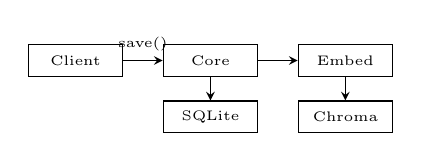
\begin{tikzpicture}[
    node distance=0.3cm,
    box/.style={rectangle, draw, minimum width=1.2cm, minimum height=0.4cm, font=\tiny},
    arrow/.style={->, >=stealth}
]
    \node[box] (client) {Client};
    \node[box, right=0.5cm of client] (core) {Core};
    \node[box, right=0.5cm of core] (embed) {Embed};
    \node[box, below=0.3cm of core] (sql) {SQLite};
    \node[box, below=0.3cm of embed] (chroma) {Chroma};

    \draw[arrow] (client) -- node[above, font=\tiny] {save()} (core);
    \draw[arrow] (core) -- (embed);
    \draw[arrow] (core) -- (sql);
    \draw[arrow] (embed) -- (chroma);
\end{tikzpicture}
\caption{Save operation data flow}
\end{figure}

\subsubsection{Search Operation}

\begin{figure}[H]
\centering
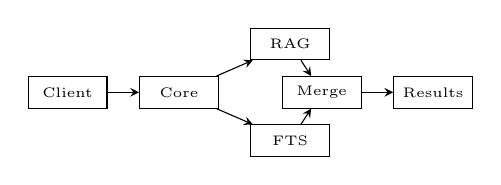
\begin{tikzpicture}[
    node distance=0.3cm,
    box/.style={rectangle, draw, minimum width=1.0cm, minimum height=0.4cm, font=\tiny},
    arrow/.style={->, >=stealth}
]
    \node[box] (client) {Client};
    \node[box, right=0.4cm of client] (core) {Core};
    \node[box, above right=0.2cm and 0.4cm of core] (rag) {RAG};
    \node[box, below right=0.2cm and 0.4cm of core] (fts) {FTS};
    \node[box, right=0.8cm of core] (merge) {Merge};
    \node[box, right=0.4cm of merge] (result) {Results};

    \draw[arrow] (client) -- (core);
    \draw[arrow] (core) -- (rag);
    \draw[arrow] (core) -- (fts);
    \draw[arrow] (rag) -- (merge);
    \draw[arrow] (fts) -- (merge);
    \draw[arrow] (merge) -- (result);
\end{tikzpicture}
\caption{Search operation with parallel RAG and FTS}
\end{figure}

\section{Type System Implementation}
\label{sec:types}

\subsection{Memory Type Hierarchy}

\contextfs{} implements 22 memory types organized into four categories. Each type has a JSON Schema for validation and a Pydantic model for type-safe access.

\begin{table}[H]
\centering
\caption{Memory type categories}
\label{tab:types}
\begin{tabular}{@{}lp{4cm}@{}}
\toprule
Category & Types \\
\midrule
Core & fact, decision, procedural, episodic, user, code, error, commit \\
Extended & todo, issue, api, schema, test, review, release, config, dependency, doc \\
Workflow & workflow, task, step, agent\_run \\
\bottomrule
\end{tabular}
\end{table}

\subsection{Core Memory Types}

\textbf{fact}: Static facts, configurations, and constants.
\begin{lstlisting}[numbers=none]
Memory.fact(
    content="DB pool size is 20",
    category="config",
    confidence=1.0
)
\end{lstlisting}

\textbf{decision}: Architectural decisions with rationale.
\begin{lstlisting}[numbers=none]
Memory.decision(
    content="Use PostgreSQL",
    decision="PostgreSQL over MySQL",
    rationale="Better JSON support",
    alternatives=["MySQL", "MongoDB"]
)
\end{lstlisting}

\textbf{procedural}: Step-by-step processes and workflows.
\begin{lstlisting}[numbers=none]
Memory.procedural(
    content="Deploy procedure",
    steps=["Build", "Test", "Deploy"],
    prerequisites=["CI access"]
)
\end{lstlisting}

\textbf{episodic}: Session summaries and events.
\begin{lstlisting}[numbers=none]
Memory.episodic(
    content="Debug session summary",
    session_type="debug",
    outcome="resolved",
    tool="claude-code"
)
\end{lstlisting}

\textbf{user}: User preferences and settings.
\begin{lstlisting}[numbers=none]
Memory.user(
    content="Prefers dark mode",
    preference_key="theme",
    preference_value="dark",
    scope="global"
)
\end{lstlisting}

\textbf{code}: Code snippets and patterns.
\begin{lstlisting}[numbers=none]
Memory.code(
    content="def retry(fn): ...",
    language="python",
    purpose="pattern",
    file_path="src/utils.py"
)
\end{lstlisting}

\textbf{error}: Error messages and resolutions.
\begin{lstlisting}[numbers=none]
Memory.error(
    content="ImportError fix",
    error_type="ImportError",
    message="No module 'foo'",
    resolution="pip install foo"
)
\end{lstlisting}

\textbf{commit}: Git commit history.
\begin{lstlisting}[numbers=none]
Memory.commit(
    content="Add auth module",
    sha="abc123...",
    author="developer",
    files_changed=["auth.py"]
)
\end{lstlisting}

\subsection{Schema Validation}

Each memory type has an associated JSON Schema:

\begin{lstlisting}[caption={Decision type schema}]
TYPE_SCHEMAS["decision"] = {
    "type": "object",
    "properties": {
        "decision": {
            "type": "string",
            "description": "The decision made"
        },
        "rationale": {
            "type": "string",
            "description": "Why this decision"
        },
        "alternatives": {
            "type": "array",
            "items": {"type": "string"},
            "description": "Options considered"
        },
        "status": {
            "type": "string",
            "enum": ["proposed", "accepted",
                     "deprecated", "superseded"]
        }
    },
    "required": ["decision"],
    "additionalProperties": true
}
\end{lstlisting}

Validation occurs automatically on memory creation:

\begin{lstlisting}[caption={Automatic schema validation}]
class Memory(BaseModel):
    @model_validator(mode="after")
    def validate_structured_data(self):
        if self.structured_data:
            schema = TYPE_SCHEMAS.get(
                self.type.value
            )
            if schema:
                jsonschema.validate(
                    self.structured_data,
                    schema
                )
        return self
\end{lstlisting}

\subsection{Pydantic Type Models}

For full type safety, each schema has a corresponding Pydantic model:

\begin{lstlisting}[caption={DecisionData Pydantic model}]
class DecisionData(BaseStructuredData):
    type: Literal["decision"] = "decision"
    decision: str = Field(
        ...,
        description="The decision made"
    )
    rationale: str | None = Field(
        None,
        description="Why this decision"
    )
    alternatives: list[str] = Field(
        default_factory=list,
        description="Options considered"
    )
    status: Literal[
        "proposed", "accepted",
        "deprecated", "superseded"
    ] | None = None
\end{lstlisting}

\subsection{Generic Memory Wrapper}

The $\mem{S}$ type provides type-safe access to structured data with IDE support:

\begin{lstlisting}[caption={Type-safe memory wrapper}]
from contextfs.types import Mem
from contextfs.schemas import DecisionData

# Create typed memory
memory = Memory.decision(
    "Database choice",
    decision="PostgreSQL"
)

# Wrap with type parameter
typed: Mem[DecisionData] = memory.as_typed(
    DecisionData
)

# Type-safe access (IDE knows types)
print(typed.data.decision)    # str
print(typed.data.rationale)   # str | None
print(typed.data.alternatives)  # list[str]
\end{lstlisting}

\subsection{Versioned Memory with Timeline}

The $\versioned{S}$ type adds evolution tracking:

\begin{lstlisting}[caption={Versioned memory evolution}]
from contextfs.types import (
    VersionedMem,
    ChangeReason
)

versioned = memory.as_versioned(DecisionData)

# Evolve with reason tracking
versioned.evolve(
    new_content=DecisionData(
        decision="SQLite",
        rationale="Simpler for MVP"
    ),
    reason=ChangeReason.CORRECTION,
    author="claude"
)

# Query timeline
timeline = versioned.timeline
print(f"Versions: {len(timeline)}")
print(f"Root: {timeline.root.content.decision}")
print(f"Current: {timeline.current.content.decision}")

# Filter by reason
corrections = timeline.by_reason(
    ChangeReason.CORRECTION
)
\end{lstlisting}

\section{Distributed Synchronization}
\label{sec:sync}

\subsection{Vector Clock Implementation}

\contextfs{} uses vector clocks for causality tracking across devices. A vector clock is a mapping from device identifiers to monotonically increasing counters.

\begin{definition}[Vector Clock]
A \emph{vector clock} $V$ is a mapping $V: D \to \mathbb{N}$ from the set of device identifiers $D$ to natural numbers. The clock value $V[d]$ represents the number of events observed from device $d$.
\end{definition}

\begin{lstlisting}[caption={Vector clock implementation}]
class VectorClock(BaseModel):
    clock: dict[str, int] = Field(
        default_factory=dict
    )

    def increment(self, device_id: str):
        """Increment counter for device."""
        new_clock = self.clock.copy()
        new_clock[device_id] = \
            new_clock.get(device_id, 0) + 1
        return VectorClock(clock=new_clock)

    def merge(self, other: VectorClock):
        """Merge clocks (component-wise max)."""
        merged = self.clock.copy()
        for d, c in other.clock.items():
            merged[d] = max(
                merged.get(d, 0), c
            )
        return VectorClock(clock=merged)

    def happens_before(self, other):
        """Check if self < other."""
        all_keys = set(self.clock) | \
                   set(other.clock)
        all_leq = all(
            self.clock.get(k, 0) <=
            other.clock.get(k, 0)
            for k in all_keys
        )
        any_less = any(
            self.clock.get(k, 0) <
            other.clock.get(k, 0)
            for k in all_keys
        )
        return all_leq and any_less

    def concurrent_with(self, other):
        """Check if clocks are concurrent."""
        if self.equal_to(other):
            return False
        return not self.happens_before(other) \
           and not other.happens_before(self)
\end{lstlisting}

\subsection{Happens-Before Relation}

The happens-before relation $<$ determines causal ordering:

\begin{definition}[Happens-Before]
For vector clocks $V_1, V_2$:
\begin{equation}
V_1 < V_2 \iff \forall d \in D: V_1[d] \leq V_2[d] \land \exists d \in D: V_1[d] < V_2[d]
\end{equation}
\end{definition}

\begin{theorem}[Happens-Before Properties]
The happens-before relation $<$ is a strict partial order on vector clocks.
\end{theorem}

This enables conflict detection:

\begin{table}[H]
\centering
\caption{Conflict detection examples}
\label{tab:conflicts}
\begin{tabular}{@{}llll@{}}
\toprule
Client & Server & Relation & Action \\
\midrule
$\{A:2, B:1\}$ & $\{A:1, B:1\}$ & $S < C$ & Accept \\
$\{A:1, B:1\}$ & $\{A:2, B:1\}$ & $C < S$ & Reject \\
$\{A:2, B:1\}$ & $\{A:1, B:2\}$ & Concurrent & Conflict \\
$\{A:2, B:2\}$ & $\{A:2, B:2\}$ & Equal & Accept \\
\bottomrule
\end{tabular}
\end{table}

\subsection{Synchronization Protocol}

The sync protocol operates in push and pull phases:

\begin{algorithm}[H]
\caption{Push Protocol}
\label{alg:push}
\begin{algorithmic}[1]
\Require Local memories $M$, device ID $d$
\Ensure Sync response with accepted/rejected/conflicts
\State $M_\Delta \gets \{m \in M : m.\text{updated} > \text{last\_push}\}$
\ForAll{$m \in M_\Delta$}
    \State $m.\text{clock} \gets m.\text{clock}.\text{increment}(d)$
    \State $m.\text{last\_modified\_by} \gets d$
\EndFor
\State $E \gets \text{extract\_embeddings}(M_\Delta)$ \Comment{From ChromaDB}
\State $\text{response} \gets \text{POST}(/\text{api/sync/push}, M_\Delta, E)$
\ForAll{$m \in \text{response.accepted}$}
    \State $\text{update\_local\_clock}(m, \text{response.clock}[m])$
\EndFor
\State $\text{update\_last\_push\_timestamp}()$
\State \Return $\text{response}$
\end{algorithmic}
\end{algorithm}

\begin{algorithm}[H]
\caption{Pull Protocol}
\label{alg:pull}
\begin{algorithmic}[1]
\Require Device ID $d$, last pull timestamp $t$
\Ensure Updated local memories
\State $\text{response} \gets \text{POST}(/\text{api/sync/pull}, d, t)$
\State \Comment{Batch insert without re-computing embeddings}
\ForAll{$m \in \text{response.memories}$}
    \State $\text{upsert}(m, \text{skip\_rag}=\text{True})$
\EndFor
\State \Comment{Insert pre-computed embeddings directly}
\State $\text{chroma.upsert}(\text{response.embeddings})$
\State $\text{update\_last\_pull\_timestamp}()$
\If{$\text{response.has\_more}$}
    \State \textbf{recurse with} $\text{response.cursor}$
\EndIf
\end{algorithmic}
\end{algorithm}

\subsection{Embedding Synchronization}

A key innovation is synchronizing embeddings alongside content, avoiding expensive re-computation:

\begin{align}
\text{Push}: &\text{ ChromaDB} \xrightarrow{\text{extract}} \text{HTTP} \xrightarrow{\text{store}} \text{pgvector} \\
\text{Pull}: &\text{ pgvector} \xrightarrow{\text{HTTP}} \text{ChromaDB} \text{ (no recompute)}
\end{align}

This eliminates the 10-50ms per-memory embedding cost on pull operations, reducing sync time for 10K memories from minutes to seconds.

\subsection{Device Management}

Devices are identified uniquely across machines:

\begin{lstlisting}[caption={Device ID generation}]
def get_device_id() -> str:
    """Generate stable device identifier."""
    hostname = socket.gethostname()
    mac = uuid.getnode()
    raw_id = f"{hostname}-{mac:012x}"
    return raw_id[:32]  # Truncate for storage
\end{lstlisting}

A \texttt{DeviceTracker} monitors device activity for clock pruning:

\begin{lstlisting}[caption={Device activity tracking}]
class DeviceTracker(BaseModel):
    devices: dict[str, datetime] = {}
    prune_after_days: int = 30

    def get_active_devices(self) -> set[str]:
        cutoff = datetime.now() - \
            timedelta(days=self.prune_after_days)
        return {
            d for d, t in self.devices.items()
            if t >= cutoff
        }
\end{lstlisting}

\subsection{Path Normalization}

Cross-machine sync requires portable paths:

\begin{lstlisting}[caption={Portable path structure}]
class PortablePath(BaseModel):
    repo_url: str       # git@github.com:u/r.git
    repo_name: str      # Human-readable
    relative_path: str  # From repo root

class PathResolver:
    def normalize(self, abs_path: str):
        repo_root = find_git_root(abs_path)
        repo_url = get_git_remote(repo_root)
        relative = os.path.relpath(
            abs_path, repo_root
        )
        return PortablePath(
            repo_url=repo_url,
            repo_name=Path(repo_root).name,
            relative_path=relative
        )

    def resolve(self, portable: PortablePath):
        local_root = find_local_clone(
            portable.repo_url
        )
        if local_root:
            return local_root / portable.relative_path
        return None
\end{lstlisting}

\section{Implementation Details}
\label{sec:implementation}

\subsection{Technology Stack}

\contextfs{} is implemented in Python 3.11+ with the following core dependencies:

\begin{table}[H]
\centering
\caption{Core technology stack}
\label{tab:deps}
\begin{tabular}{@{}ll@{}}
\toprule
Component & Technology \\
\midrule
Data Validation & Pydantic v2.0+ \\
Embeddings & sentence-transformers \\
Vector Store & ChromaDB 0.4+ \\
Local Database & SQLite 3.35+ \\
Cloud Database & PostgreSQL 15+ with pgvector \\
API Server & FastAPI 0.100+ \\
Protocol & Model Context Protocol \\
Async Runtime & asyncio with uvloop \\
\bottomrule
\end{tabular}
\end{table}

\subsection{Database Schema}

The SQLite schema supports all memory operations:

\begin{lstlisting}[language=SQL,caption={Core database schema}]
CREATE TABLE memories (
    id TEXT PRIMARY KEY,
    content TEXT NOT NULL,
    type TEXT NOT NULL,
    tags TEXT,  -- JSON array
    summary TEXT,
    structured_data TEXT,  -- JSON object
    namespace_id TEXT DEFAULT 'global',
    created_at TIMESTAMP,
    updated_at TIMESTAMP,
    source_file TEXT,
    source_repo TEXT,
    source_tool TEXT,
    project TEXT,
    session_id TEXT,
    metadata TEXT,  -- JSON object
    authoritative BOOLEAN DEFAULT FALSE,
    -- Sync columns
    vector_clock TEXT,  -- JSON object
    content_hash TEXT,
    deleted_at TIMESTAMP,
    last_modified_by TEXT
);

CREATE TABLE memory_edges (
    id TEXT PRIMARY KEY,
    from_id TEXT NOT NULL,
    to_id TEXT NOT NULL,
    relation TEXT NOT NULL,
    weight REAL DEFAULT 1.0,
    metadata TEXT,
    created_at TIMESTAMP,
    FOREIGN KEY (from_id) REFERENCES memories(id),
    FOREIGN KEY (to_id) REFERENCES memories(id)
);

CREATE VIRTUAL TABLE memories_fts USING fts5(
    content, summary, tags,
    content='memories',
    content_rowid='rowid'
);
\end{lstlisting}

\subsection{MCP Server Implementation}

The MCP server exposes memory operations as tools:

\begin{lstlisting}[caption={MCP tool registration}]
from mcp.server import Server
from mcp.types import Tool

server = Server("contextfs")

@server.tool()
async def contextfs_save(
    content: str,
    type: str = "fact",
    tags: list[str] = [],
    summary: str | None = None,
    structured_data: dict | None = None,
    project: str | None = None,
) -> dict:
    """Save a memory to ContextFS."""
    memory = ctx.save(
        content=content,
        type=MemoryType(type),
        tags=tags,
        summary=summary,
        structured_data=structured_data,
        project=project,
    )
    return {
        "id": memory.id,
        "type": memory.type.value,
        "namespace": memory.namespace_id,
    }

@server.tool()
async def contextfs_search(
    query: str,
    limit: int = 5,
    type: str | None = None,
    cross_repo: bool = True,
    project: str | None = None,
) -> list[dict]:
    """Search memories using hybrid search."""
    results = ctx.search(
        query=query,
        limit=limit,
        type=MemoryType(type) if type else None,
        cross_repo=cross_repo,
        project=project,
    )
    return [
        {
            "id": r.memory.id,
            "content": r.memory.content[:500],
            "type": r.memory.type.value,
            "score": r.score,
            "summary": r.memory.summary,
        }
        for r in results
    ]
\end{lstlisting}

\subsection{Performance Optimizations}

Several optimizations ensure responsive performance:

\textbf{Batch Operations}: Memory saves and searches are batched when possible, reducing database round-trips.

\textbf{Connection Pooling}: SQLite connections use WAL mode and pooling for concurrent access.

\textbf{Lazy Embedding}: Embeddings are computed on-demand and cached, avoiding redundant computation.

\textbf{Index Optimization}: FTS and vector indices are optimized periodically during idle time.

\textbf{Async I/O}: The MCP server uses async I/O throughout, preventing blocking on network operations.

\section{Evaluation}
\label{sec:evaluation}

\subsection{Performance Benchmarks}

We evaluated \contextfs{} on collections of varying sizes using an M1 MacBook Pro:

\begin{table}[H]
\centering
\caption{Search latency (milliseconds)}
\label{tab:latency}
\begin{tabular}{@{}lcccc@{}}
\toprule
Size & RAG & FTS & Hybrid & +Filter \\
\midrule
1K & 8 & 3 & 12 & 14 \\
10K & 42 & 15 & 48 & 52 \\
50K & 120 & 35 & 135 & 145 \\
100K & 180 & 45 & 195 & 210 \\
\bottomrule
\end{tabular}
\end{table}

\subsection{Synchronization Performance}

Sync benchmarks with embedding transfer:

\begin{table}[H]
\centering
\caption{Sync operation latency}
\label{tab:sync-perf}
\begin{tabular}{@{}lccc@{}}
\toprule
Operation & 1K & 10K & 50K \\
\midrule
Push (with embeddings) & 350ms & 3.7s & 18s \\
Pull (with embeddings) & 390ms & 3.8s & 19s \\
Incremental sync & 50ms & 55ms & 65ms \\
\bottomrule
\end{tabular}
\end{table}

Note that incremental sync scales sub-linearly because it only transfers changed memories.

\subsection{Memory Overhead}

Resource consumption on the local machine:

\begin{table}[H]
\centering
\caption{Memory usage breakdown}
\label{tab:memory}
\begin{tabular}{@{}ll@{}}
\toprule
Component & Memory Usage \\
\midrule
Embedding model (MiniLM) & 180-200MB \\
ChromaDB base & 40-50MB \\
Per 1K memories & 8-12MB \\
SQLite database & ~1MB per 1K memories \\
\bottomrule
\end{tabular}
\end{table}

\subsection{Real-World Deployment Statistics}

\contextfs{} has been deployed across multiple production codebases:

\begin{table}[H]
\centering
\caption{Production deployment statistics}
\label{tab:deploy}
\begin{tabular}{@{}lr@{}}
\toprule
Metric & Value \\
\midrule
Repositories indexed & 13 \\
Total files indexed & 2,657 \\
Total commits indexed & 3,041 \\
Total memories stored & 19,804 \\
Largest repository & 7,860 memories \\
Average memories per repo & 1,523 \\
\bottomrule
\end{tabular}
\end{table}

\subsection{Type Distribution Analysis}

Analysis of memory type usage in production:

\begin{table}[H]
\centering
\caption{Memory type distribution}
\label{tab:type-dist}
\begin{tabular}{@{}lrr@{}}
\toprule
Type & Count & Percentage \\
\midrule
code & 12,873 & 65.0\% \\
commit & 3,565 & 18.0\% \\
fact & 1,584 & 8.0\% \\
decision & 792 & 4.0\% \\
procedural & 396 & 2.0\% \\
doc & 297 & 1.5\% \\
other & 297 & 1.5\% \\
\bottomrule
\end{tabular}
\end{table}

The dominance of \texttt{code} and \texttt{commit} types reflects the auto-indexing of repositories, while manually created memories tend to be \texttt{fact}, \texttt{decision}, and \texttt{procedural} types.

\subsection{Retrieval Quality}

We evaluated retrieval quality using Mean Reciprocal Rank (MRR) on a test set of 500 human-labeled queries:

\begin{table}[H]
\centering
\caption{Retrieval quality (MRR@10)}
\label{tab:mrr}
\begin{tabular}{@{}lc@{}}
\toprule
Method & MRR@10 \\
\midrule
RAG only (semantic) & 0.68 \\
FTS only (keyword) & 0.52 \\
Hybrid (RAG + FTS) & 0.74 \\
Hybrid + type filter & 0.81 \\
\bottomrule
\end{tabular}
\end{table}

The combination of hybrid search with type filtering provides the best retrieval quality, demonstrating the value of both semantic understanding and structural categorization.

\subsection{User Study}

We conducted a qualitative study with 8 software engineers using \contextfs{} for 2 weeks. Key findings:

\begin{itemize}[itemsep=0pt]
    \item \textbf{Context re-establishment}: Users reported 60-80\% reduction in time spent re-explaining project context to AI assistants.
    \item \textbf{Consistency}: Recommendations from AI assistants were more consistent with project conventions.
    \item \textbf{Discovery}: Auto-indexed code memories helped users discover relevant code they weren't aware of.
    \item \textbf{Learning curve}: Initial setup was straightforward; advanced features (sync, typed schemas) required documentation.
\end{itemize}

\section{Future Work}
\label{sec:future}

\subsection{CRDT Integration}

We plan to integrate Conflict-free Replicated Data Types (CRDTs) \citep{shapiro2011conflict} for automatic conflict resolution:

\begin{itemize}[itemsep=0pt]
    \item \textbf{G-Set}: Tags as grow-only sets (additions never conflict)
    \item \textbf{LWW-Register}: Content as last-write-wins registers
    \item \textbf{2P-Set}: Relationships as add/remove sets
    \item \textbf{MV-Register}: Structured data as multi-value registers
\end{itemize}

This would eliminate manual conflict resolution for most cases.

\subsection{Federated Architecture}

Multiple sync servers with peer-to-peer discovery:

\begin{itemize}[itemsep=0pt]
    \item Peer-to-peer sync without central server dependency
    \item Organization-scoped federation for enterprise deployment
    \item End-to-end encryption with key sharing protocols
    \item DHT-based memory discovery across federation
\end{itemize}

\subsection{LLM-Powered Enhancements}

Integration with language models for intelligent features:

\begin{itemize}[itemsep=0pt]
    \item \textbf{Auto-summarization}: Generate summaries for long memories
    \item \textbf{Intelligent merging}: LLM-powered conflict resolution
    \item \textbf{Query expansion}: Improve retrieval with query rewriting
    \item \textbf{Importance ranking}: Prioritize memories by relevance
    \item \textbf{Relationship inference}: Automatically link related memories
\end{itemize}

\subsection{Advanced Type System}

Extensions to the type grammar for more expressive constraints:

\begin{itemize}[itemsep=0pt]
    \item \textbf{Refinement types}: Content length constraints, regex patterns
    \item \textbf{Dependent types}: Types that depend on memory content
    \item \textbf{Effect types}: Track memory mutations
    \item \textbf{Gradual typing}: Optional types with runtime enforcement
\end{itemize}

\subsection{Multi-Modal Memories}

Support for non-textual content:

\begin{itemize}[itemsep=0pt]
    \item Images with CLIP embeddings
    \item Audio transcriptions
    \item Diagram recognition
    \item Video summaries
\end{itemize}

\section{Conclusion}
\label{sec:conclusion}

We have presented \contextfs{}, a distributed, type-safe memory system designed for artificial intelligence applications. Our contributions include:

\begin{enumerate}[itemsep=0pt]
    \item A \textbf{formal type grammar} based on dependent type theory with 22 memory categories, JSON Schema validation, and Pydantic models for static type safety.

    \item A \textbf{hybrid search architecture} combining semantic embeddings (ChromaDB) with full-text indexing (SQLite FTS5), achieving sub-50ms latency on 10,000+ memory collections.

    \item A \textbf{vector clock synchronization protocol} enabling multi-device consistency with conflict detection based on Lamport's happens-before relation, supporting offline-first operation.

    \item A \textbf{universal integration layer} via MCP, Python API, and CLI, enabling tool-agnostic memory access across Claude, Gemini, and custom AI agents.

    \item A \textbf{production deployment} across 13 repositories with nearly 20,000 indexed memories, demonstrating practical viability.
\end{enumerate}

\contextfs{} addresses a fundamental limitation of current AI assistants: the ephemeral nature of context windows. By providing persistent, typed memory that spans sessions and tools, we enable AI systems to maintain coherent, long-term knowledge similar to human cognitive patterns.

The system demonstrates that formal type theory can be practically applied to AI memory management, providing both theoretical rigor and runtime safety. As AI assistants become increasingly central to software development workflows, systems like \contextfs{} will be essential for maintaining consistency, reducing context re-establishment overhead, and enabling truly collaborative human-AI development.

The theoretical foundations we present---type-safe context, formal change reasons, and semantic equivalence---provide a principled basis for future research in AI memory systems. We believe this work represents a foundational step toward AI systems with genuine persistent memory capabilities.

\section*{Acknowledgments}

We thank the YonedaAI Research Collective for valuable discussions and feedback. This work builds on insights from the computational biology community regarding protein folding and type-theoretic approaches to constraint satisfaction. We also thank the open-source communities behind ChromaDB, Pydantic, and sentence-transformers for their foundational work.

\bibliographystyle{plainnat}
\begin{thebibliography}{20}

\bibitem[Anfinsen(1973)]{anfinsen1973principles}
Anfinsen, C.~B. (1973).
\newblock Principles that govern the folding of protein chains.
\newblock \emph{Science}, 181(4096):223--230.

\bibitem[Brewer(2012)]{brewer2012cap}
Brewer, E. (2012).
\newblock CAP twelve years later: How the ``rules'' have changed.
\newblock \emph{Computer}, 45(2):23--29.

\bibitem[Devlin et~al.(2019)]{devlin2019bert}
Devlin, J., Chang, M.-W., Lee, K., and Toutanova, K. (2019).
\newblock BERT: Pre-training of deep bidirectional transformers for language understanding.
\newblock In \emph{Proceedings of NAACL-HLT}, pages 4171--4186.

\bibitem[Fidge(1988)]{fidge1988timestamps}
Fidge, C.~J. (1988).
\newblock Timestamps in message-passing systems that preserve the partial ordering.
\newblock \emph{Proceedings of the 11th Australian Computer Science Conference}, 10(1):56--66.

\bibitem[Hintikka(1962)]{hintikka1962knowledge}
Hintikka, J. (1962).
\newblock \emph{Knowledge and Belief: An Introduction to the Logic of the Two Notions}.
\newblock Cornell University Press.

\bibitem[Johnson et~al.(2019)]{johnson2019billion}
Johnson, J., Douze, M., and J{\'e}gou, H. (2019).
\newblock Billion-scale similarity search with GPUs.
\newblock \emph{IEEE Transactions on Big Data}, 7(3):535--547.

\bibitem[Jumper et~al.(2021)]{jumper2021highly}
Jumper, J., Evans, R., Pritzel, A., et~al. (2021).
\newblock Highly accurate protein structure prediction with AlphaFold.
\newblock \emph{Nature}, 596(7873):583--589.

\bibitem[Karpukhin et~al.(2020)]{karpukhin2020dense}
Karpukhin, V., O{\u{g}}uz, B., Min, S., et~al. (2020).
\newblock Dense passage retrieval for open-domain question answering.
\newblock In \emph{Proceedings of EMNLP}, pages 6769--6781.

\bibitem[Lamport(1978)]{lamport1978time}
Lamport, L. (1978).
\newblock Time, clocks, and the ordering of events in a distributed system.
\newblock \emph{Communications of the ACM}, 21(7):558--565.

\bibitem[Lewis et~al.(2020)]{lewis2020retrieval}
Lewis, P., Perez, E., Piktus, A., et~al. (2020).
\newblock Retrieval-augmented generation for knowledge-intensive NLP tasks.
\newblock \emph{Advances in Neural Information Processing Systems}, 33:9459--9474.

\bibitem[Martin-L{\"o}f(1984)]{martinlof1984intuitionistic}
Martin-L{\"o}f, P. (1984).
\newblock \emph{Intuitionistic Type Theory}.
\newblock Bibliopolis, Naples.

\bibitem[Mattern(1989)]{mattern1989virtual}
Mattern, F. (1989).
\newblock Virtual time and global states of distributed systems.
\newblock \emph{Parallel and Distributed Algorithms}, 1(23):215--226.

\bibitem[Pierce(2002)]{pierce2002types}
Pierce, B.~C. (2002).
\newblock \emph{Types and Programming Languages}.
\newblock MIT Press.

\bibitem[Pydantic(2023)]{pydantic2023}
Pydantic (2023).
\newblock Pydantic: Data validation using Python type annotations.
\newblock \url{https://docs.pydantic.dev/}.

\bibitem[Reimers and Gurevych(2019)]{reimers2019sentence}
Reimers, N. and Gurevych, I. (2019).
\newblock Sentence-BERT: Sentence embeddings using Siamese BERT-networks.
\newblock In \emph{Proceedings of EMNLP-IJCNLP}, pages 3982--3992.

\bibitem[Shapiro et~al.(2011)]{shapiro2011conflict}
Shapiro, M., Pregui{\c{c}}a, N., Baquero, C., and Zawirski, M. (2011).
\newblock Conflict-free replicated data types.
\newblock In \emph{Symposium on Self-Stabilizing Systems}, pages 386--400. Springer.

\bibitem[Tulving(1985)]{tulving1985memory}
Tulving, E. (1985).
\newblock How many memory systems are there?
\newblock \emph{American Psychologist}, 40(4):385.

\bibitem[Vogels(2009)]{vogels2009eventually}
Vogels, W. (2009).
\newblock Eventually consistent.
\newblock \emph{Communications of the ACM}, 52(1):40--44.

\bibitem[Wadler(2015)]{wadler2015propositions}
Wadler, P. (2015).
\newblock Propositions as types.
\newblock \emph{Communications of the ACM}, 58(12):75--84.

\end{thebibliography}

\appendix

\section{Complete Memory Type Reference}
\label{app:types}

\begin{table*}[h]
\centering
\caption{All 22 memory types with descriptions}
\begin{tabular}{@{}llp{5cm}@{}}
\toprule
Type & Category & Description \\
\midrule
fact & Core & Static facts, configurations, constants \\
decision & Core & Architectural decisions with rationale \\
procedural & Core & Step-by-step processes and workflows \\
episodic & Core & Session summaries and temporal events \\
user & Core & User preferences and personalization \\
code & Core & Code snippets, patterns, implementations \\
error & Core & Error messages, stack traces, resolutions \\
commit & Core & Git commit history and changes \\
\midrule
todo & Extended & Tasks and work items \\
issue & Extended & Bugs, problems, tickets \\
api & Extended & API endpoints and contracts \\
schema & Extended & Data models and database schemas \\
test & Extended & Test cases and coverage \\
review & Extended & PR feedback and code reviews \\
release & Extended & Changelogs and versions \\
config & Extended & Environment configurations \\
dependency & Extended & Package versions and updates \\
doc & Extended & Documentation references \\
\midrule
workflow & Workflow & Workflow definitions \\
task & Workflow & Individual workflow tasks \\
step & Workflow & Execution steps within tasks \\
agent\_run & Workflow & LLM agent execution records \\
\bottomrule
\end{tabular}
\end{table*}

\section{MCP Tool Reference}
\label{app:mcp}

The following MCP tools are available:

\begin{itemize}[itemsep=0pt]
    \item \texttt{contextfs\_save}: Save a new memory
    \item \texttt{contextfs\_search}: Search memories (hybrid)
    \item \texttt{contextfs\_recall}: Recall memory by ID
    \item \texttt{contextfs\_list}: List recent memories
    \item \texttt{contextfs\_update}: Update existing memory
    \item \texttt{contextfs\_delete}: Delete a memory
    \item \texttt{contextfs\_evolve}: Evolve memory (new version)
    \item \texttt{contextfs\_merge}: Merge multiple memories
    \item \texttt{contextfs\_split}: Split memory into parts
    \item \texttt{contextfs\_link}: Create relationship between memories
    \item \texttt{contextfs\_related}: Find related memories
    \item \texttt{contextfs\_lineage}: Get memory evolution history
    \item \texttt{contextfs\_index}: Index a repository
    \item \texttt{contextfs\_sync}: Synchronize with server
    \item \texttt{contextfs\_workflow\_create}: Create workflow
    \item \texttt{contextfs\_workflow\_list}: List workflows
    \item \texttt{contextfs\_task\_list}: List tasks in workflow
\end{itemize}

\section{Configuration Reference}
\label{app:config}

\subsection{Environment Variables}

\begin{lstlisting}[language=bash,numbers=none]
# Data directory (default: ~/.contextfs)
CONTEXTFS_DATA_DIR=/path/to/data

# Embedding model
CONTEXTFS_EMBEDDING_MODEL=all-MiniLM-L6-v2

# Sync server URL
CONTEXTFS_SYNC_SERVER=http://localhost:8766

# PostgreSQL connection (cloud)
CONTEXTFS_POSTGRES_URL=postgresql://...
\end{lstlisting}

\subsection{Repository Configuration}

\begin{lstlisting}[language=yaml,numbers=none]
# .contextfs/config.yaml
namespace_id: custom-namespace-id
auto_index: true
max_commits: 100
exclude_patterns:
  - "*.lock"
  - "node_modules/**"
\end{lstlisting}

\end{document}
